\chapter{Results}
\label{results}

Borrowing again from Flaxman 2014, the models were evaluated on a variant of $R^2$ that captures the reduction in total variance from each kernel component, which in turn can be interpreted as a measure of what components are most important in explaining the model. The error from predicting solely on the prior spatial expectation $e_s$ serves as a baseline for comparison:

$$ Reduction-in-Variance = 1 - \frac{\sigma_{s,t}(n_{s,t}- \hat{n_{s,t}})^2}{\sigma_{s,t}(n_{s,t} - e_{s})^2}$$

Mean Squared Error (MSE) was also calculated for each of the predictions from each $f_i(s,t)$ and compared to an AR(1) model that only relies on temporal predictions from the prior period. \par

A Pareto-Smoothed-Importance-Sampling Leave-One-Out score (PSIS-LOO) was used to check the fit of the variational approximation of the posterior density \cite{vehtari_loo}. The PSIS-LOO score, also referred to as $k$, is a measure for estimating the pointwise out-of-sample prediction accuracy of a model. Generally $k$ scores of less than 0.5 are desirable, with scores between 0.5 and 1 necessitating caution.


\section{Long Term Predictions}

 Weekly traffic collision and injury data was aggregated to one weekly series for all of New York City. While data is available for the past five years, there appears to have been a reporting error for part of 2016 which made the year of data problematic for both model fitting and testing \ref{AppendixA}. It would have been ideal to fit the model based on multiple years of data leading up to the latest available data, but given the unreliable data the best alternative was fitting the LGCP on three years of data from July 2012 to July 2015, and leaving the following 52 weeks for out-of-sample prediction.  Crashes without latitude and longitude were excluded, as well as any crashes that happened on highways and other high-speed motorways. The prior spatial expectation $e_s$ was taken from New York State Department of Health statistics for injuries stemming from motor vehicle collisions during the in-sample period \cite{nys_crash_stats}. \par

 Figure \ref{city_preds} shows the model fit for the citywide data:

 \begin{figure}[h!]
   \centering
   \caption{A Gaussian Process fit to weekly pedestrian injuries in New York City from 2012 to 2015. The dotted line shows where out of sample prediction begins. The 95\% credible interval - in light grey - contains less than 95\% of the observed data, which suggests the parameters may not be optimal.}
   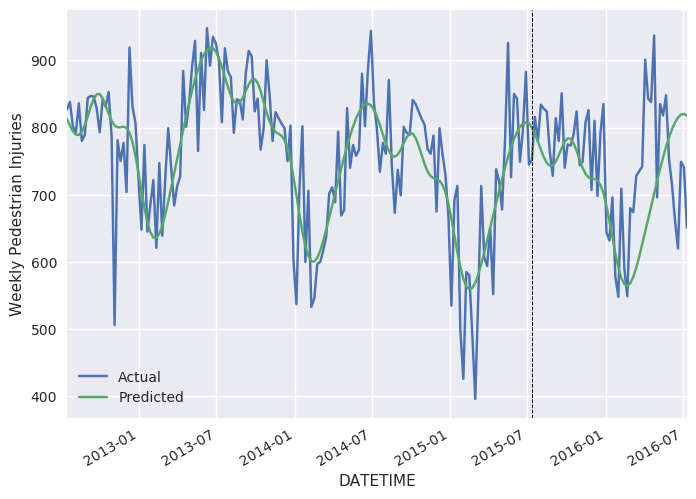
\includegraphics[width=\textwidth]{citywide_predictions}
   \label{city_preds}
 \end{figure}

\subsection{Kernel Components}

Since the kernel components are all additive they can provide an interpretable decomposition of the model components. There is clear annual periodicity in the model, which is also confirmed by the period parameter fitted being almost exactly 52. The linear kernel component also suggests a small downward long-term trend in pedestrian injuries.

\begin{table}[h!]
\centering
\caption{Models Considered}
\label{citywide_parameters}
\begin{tabular}{@{}llllll@{}}
\toprule
kernel                                      & prior                                   & value \\
PartialVGP/kern/periodic/period       & None                                    & 0.52 \\
PartialVGP/kern/periodic/variance     & student-T({[} 0.{]},{[} 1.{]}{[} 4.{]}) & 0.03  \\
PartialVGP/kern/periodic/lengthscales & student-T({[} 0.{]},{[} 1.{]}{[} 4.{]}) & 0.40  \\
PartialVGP/kern/rbf/variance          & student-T({[} 0.{]},{[} 1.{]}{[} 4.{]}) & 0.38  \\
PartialVGP/kern/rbf/lengthscales      & student-T({[} 0.{]},{[} 1.{]}{[} 4.{]}) & 0.89  \\
PartialVGP/kern/linear/variance       & student-T({[} 0.{]},{[} 1.{]}{[} 4.{]}) & 0.54
\end{tabular}
\end{table}



The Reduction-in-Variance for each kernel component shows the temporal RBF kernel captures almost all the explanatory benefit of the model by itself. Note that each kernel component was evaluated independently so the RIV of the individual components will not add up to the Combined total. \par

\begin{table}[h!]
\centering
\caption{Models Considered}
\label{variance_citywide}
\begin{tabular}{@{}llllll@{}}
\toprule
Kernel     & Reduction-in-Variance &  \\
Linear     & 43.2\%                &  \\
Time (RBF) & 85.2\%                &  \\
Periodic   & 13.5\%                &  \\
Combined   & 95.1\%                &
\end{tabular}
\end{table}

It is possible to plot the additive components of the $log(f)$ latent risk function in order to explain the final Combined total. As seen in \ref{citywide_var_decomp}, the long-term model suggests a modest downward trend in risk from traffic collisions as reflected by the linear kernel, independent of any seasonal or time-trend components. \par

\begin{figure}[h!]
  \centering
  \caption{Additive components of the latent risk function.}
  \label{citywide_var_decomp}
  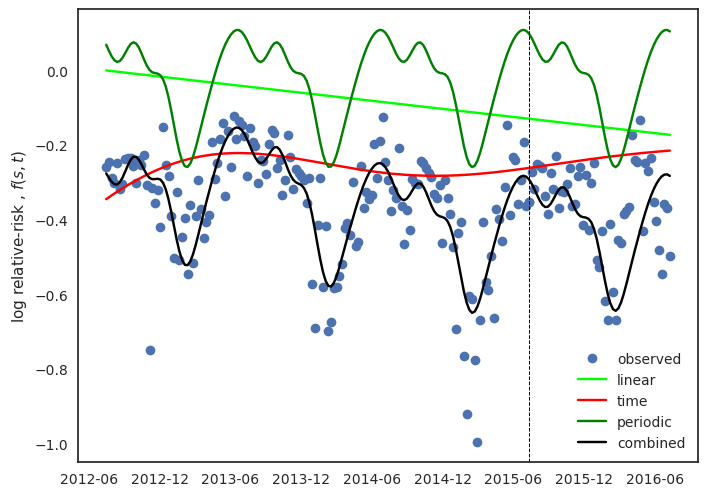
\includegraphics[width=.9\textwidth]{citywide_var_decomp}
\end{figure}

The PSIS-LOO $k$ score for the citywide model was 0.8, which is problematically high but not necessarily disqualifying according to \cite{vehtari_loo}.

 \section{Neighborhood Predictions}

 A neighborhood level model adds a spatial component to the existing temporal model.  New York City defines official Neighborhood Tabulation Areas (NTAs), which were used as the geographic areas of interest. The model was fit on the 29 official NTAs in the borough of Manhattan using 52 weeks of weekly pedestrian injury data starting in January 2013. The out-of-sample period was the first 26 weeks of 2014. Again the reporting gaps in collision data limited the periods where reliable data was available continuously for all neighborhoods. $e_s$ was calculated using the average number of weekly neighborhood pedestrian injuries prior to January 2013.  The spatial distance was calculated from the distance between centroids for each NTA (in feet) on the NAD83 New York State Plane projection. \par

 \begin{table}[h!]
\centering
\caption{NTA data example.}
\label{nta_data_table}
\begin{tabular}{@{}llllll@{}}
\toprule
   & COUNT & NTAName                           & x\_point            & y\_point            & DATETIME   \\ \midrule
4  & 0.0   & Battery Park City-Lower Manhattan & 0.0814095 & 0.0972240 & 2012-07-01 \\
20 & 0.0   & Central Harlem North-Polo Grounds & 0.1006435 & 0.1373956 & 2012-07-01 \\
21 & 1.0   & Central Harlem South              & 0.0977342 & 0.1323207 & 2012-07-01 \\
23 & 5.0   & Chinatown                         & 0.0857386 & 0.0999914 & 2012-07-01 \\
24 & 0.0   & Clinton                           & 0.0863560 & 0.1176865  & 2012-07-01 \\ \bottomrule
\end{tabular}
\end{table}



   \begin{figure}[h!]
     \centering
     \caption{Relative risk scores for Manhattan neighborhoods. Midtown is roughly twice as dangerous for pedestrians than Manhattan as a whole.}
     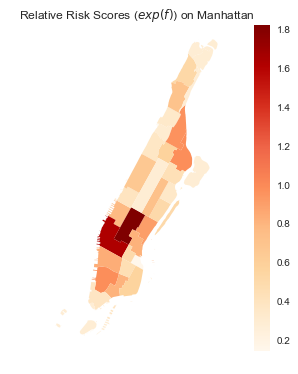
\includegraphics[\textwidth]{mn_f_score_map}
   \end{figure}


 \end{figure}


 The LGCP predictions performed as well as AR(1) models trained on each neighborhood seperately, Although the MSE for the spatiotemporal model during the out-of-sample period was slightly lower than the AR(1) model average, the difference is negligible.


  \begin{figure}[h!]
    \centering
    \caption{Average Mean Squared Error for each neighborhood during the out-of-sample period for the LGCP model and a AR(1) comparison.}
    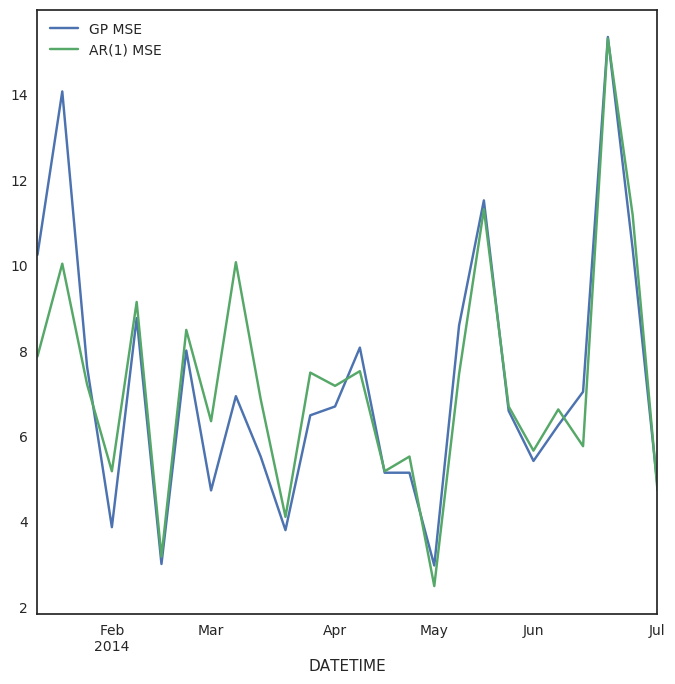
\includegraphics[width=.6\textwidth]{NTA_MSE}
  \end{figure}

  The PSIS-LOO score for the neighborhood model was close to 1 , which is worryingly large and undermines the predictive potential of the model.

  \subsection{Kernel Components}

  The neighborhood model assumes a stationary kernel in contrast to the citywide model. The two-dimensional spatial distance Matern32 kernel contributes noticeably to the Reduction-in-Variance score, while the RBF time kernel and the multiplicative interaction between space and time are also large contributors to the model's explanatory power. The Periodic component makes a smaller contribution than in the long-term model. The total Reduction-in-Variance of 65\% is less than the long term model, but still a large improvement over defaulting to neighborhood averages. \par

  \begin{table}[]
  \centering
  \caption{Neighborhood Reduction-in-Variance}
  \label{variance_neighb}
  \begin{tabular}{@{}lll@{}}
  \toprule
                     & Reduction-in-Variance &  \\ \midrule
  Time (RBF)         & 27.2\%                &  \\
  Spatial (Matern32) & 22.3\%                &  \\
  Periodic           & 2.0\%                 &  \\
  Product            & 19.2\%                &  \\
  Combined           & 64.6\%                &  \\ \bottomrule
  \end{tabular}
  \end{table}



Since the exponentiated latent function $exp(f(s,t))$ is directly interpretable as a measure of relative risk it can be used for direct comparisons between neighborhoods \par


A similar assessment of relative risk can be done across periods, A comparison between three Manhattan neighborhoods in \ref{MN_f_neighbs_example} shows varying levels of latent risk while all three are subject to seasonality and periodicity.

\begin{figure}[h!]
  \centering
  \caption{}
  \label{MN_f_neighbs_example}
  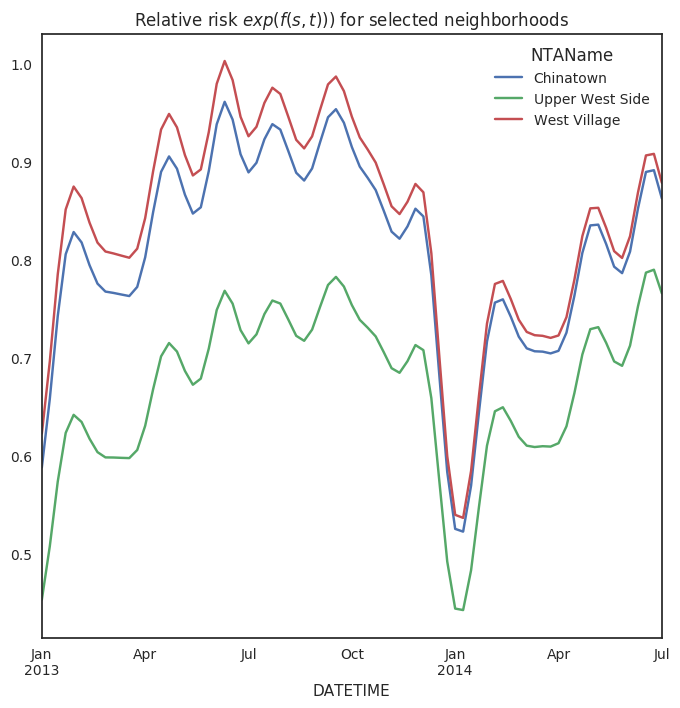
\includegraphics[width=.6\textwidth]{MN_f_neighbs_example}
\end{figure}



\section{Short Term Forecasting}

Short term forecasting using grid data was tested on a single neighborhood using weekly data. The neighborhood of Park Slope, Brooklyn was overlaid with a square grid and all data within the square was aggregated. The model included all vehicle collisions rather than only collisions causing pedestrian injuries because the data for pedestrian injuries is already quite sparse when looking at at the level of an individual neighborhood. The majority of grid squares will see no observed data for any given week. The grid model was tested with an out-of-sample period of 12 weeks while varying the historical training length between 3-12 preceding weeks. Distance was measured between the center of each grid square. The prior spatial expectation $e_s$ was taken from the average weekly collisions in Park Slope during 2015 and scaled by the number of grid squares. Figure \ref{f_risk_grid_500ft} shows a short-term model fitted to grid squares with an edge length of 500 feet. \par


\begin{figure}[h!]
  \centering
  \caption{}
  \label{f_risk_grid_500ft}
  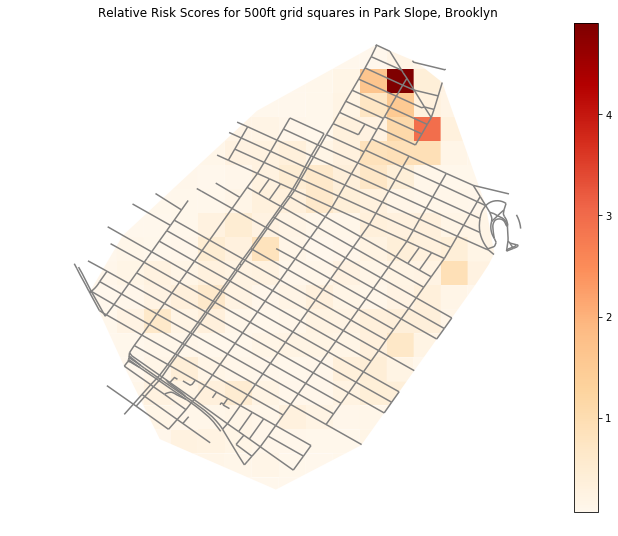
\includegraphics[width=.9\textwidth]{f_risk_grid_500ft}
\end{figure}

The short-term model outperformed an AR(1) noticeably as measured by MSE, especially when using less time periods for fitting. This can be seen in \ref{grid_MSE}. The difference in performance was especially relevant when forecasting futher into the out-of-sample period. The AR(1) performance converged to be comparable to the Gaussian Process model as the number of weeks used for fitting increased, while the PSIS-LOO score was 0.8. \par

\begin{figure}[]
  \centering
  \caption{Average Mean Squared Error across grid squares during the out-of-sample period for the LGCP model and a AR(1) comparison}
  \label{grid_MSE}
  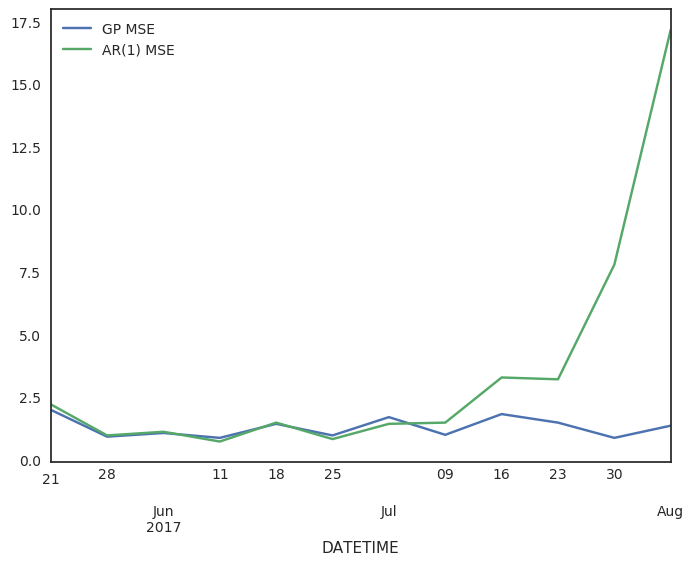
\includegraphics[width=.9\textwidth]{grid_MSE}
\end{figure}


\subsection{Kernel Components}

The kernel components were kept as close as possible to the neighborhood model, but the spatial Matern32 kernel proved to be too unstable, even after adding a jitter; another RBF kernel was used instead. The short-term model had the lowest share of explained variance between the three models, almost entirely attributable to the spatial kernel. \par

\begin{table}[]
\centering
\caption{Grid Square Model Reduction-in-Variance}
\label{variance_grid}
\begin{tabular}{@{}lll@{}}
\toprule
              & Reduction-in-Variance &  \\ \midrule
Time (RBF)    & -3.5\%                &  \\
Spatial (RBF) & 35.6\%                &  \\
Periodic      & 0.0\%                 &  \\
Product       & 26.1\%                &  \\
Combined      & 32.0\%                &  \\ \bottomrule
\end{tabular}
\end{table}
